\externaldocument{../appendix/chapter_app}
\externaldocument{../4/chapter_algorithm}
\externaldocument{../3/chapter_modeling}
\startchapter{Proof of Concept}
\label{chapter:Exp}
In this chapter, I present two experiments I ran as a proof of concept of the communication analysis of dual\_trace.

These experiments were aimed to test the communication model and the communication analysis approach. They also verify the correctness of the algorithms. I used the implemented features on Atlantis to conduct the experiments.

The selection of the experiments are restricted by the traces that can be captured. The current in-house tracer of DRDC is only able to capture the function information for some .dll files. kernel32.dll which contains the functions for Named pipe is one of the .dll files that this tracer can capture. Functions for the other communication methods discussed in this thesis can not be captured by DRDC's tracer currently.  Thus both of the conducted experiments used the named pipe communication method. 

Among these two experiments, the first one was provided directly by our research partner DRDC with their initial requirement, while I designed the second one. In both experiments, DRDC conducted the programs execution and captured the traces on their environment, while I performed the analysis locally with Atlantis on my desktop with the captured traces. All test programs in these two experiments were written in C++ and the source code can be found in Appendix \ref{expcode}. 

In both experiments, three major steps are conducted:
\begin{enumerate}
\item Execute the test programs and capture the traces for each program (done by DRDC)

\item Perform the ``Stream Exaction" and ``Communication Identification" operation on the dual\_trace

\item Manually verify the result by navigating the events in the ``Communication view" and check if they match the sequence diagrams of each experiment
\end{enumerate}

In the following two sections, I will describe the design of the experiments first and then present the result of them with discussion of each one.

\section{Experiment 1}
\subsection{Experiment Design}
In the first experiment, two programs communicated with each other through a synchronous named pipe channel. One of the programs acted as the named pipe server while the other as the client. Figure \ref{exp1} is the sequence diagram of the interaction between the server and client. This sequence diagram only exemplifies a possible sequence of the events. The actual event sequence can vary depending on the run-time environment. 


\begin{figure}[H]
\centerline{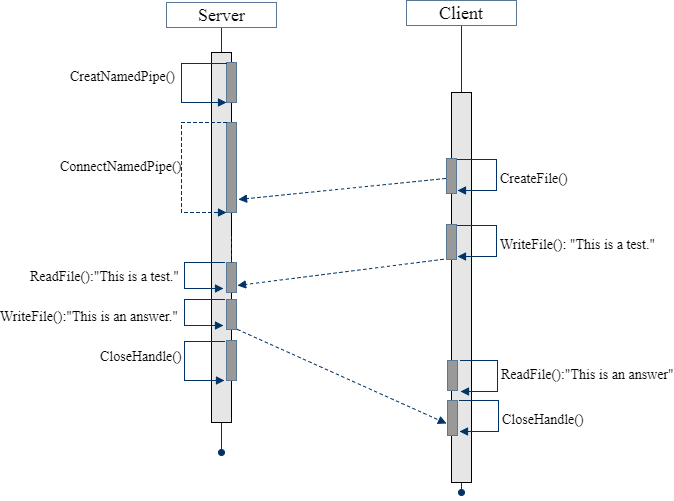
\includegraphics[scale=0.6]{Figures/exp1}}
 \caption{Sequence Diagram of Experiment 1}
\label{exp1}
\end{figure}

The traces of these programs running and interacting were captured. The two captured traces, $Sever.trace$ and $Client.trace$ were analyzed as a dual\_trace and named $dual\_trace\_1$. I performed ``Stream identification" and ``Communication identification" following the use cases in Table \ref{usecase1} and Table \ref{usecase2} with $dual\_trace\_1$ and the corresponding kernel32.dll. The function descriptor for the analysis of $dual\_trace\_1$ is shown in Table \ref{fdescexp1}.

\begin{table}[H]
  \centering
  \caption{Function Descriptor of Named Pipe for Experiment 1}
  \label{fdescexp1}
  \begin{tabular}{|l|l|l|l|l|l|l|l|}
\hline
             \multirow{2}{*}{{\textbf{Name}}} & \multirow{2}{*}{{\textbf{Type}}} & \multicolumn{3}{c|}{\textbf{Input Parameters Description}} & \multicolumn{3}{c|}{\textbf{Output Parameters Description}} \\
              \cline{3-8} 
             & & \textbf{Name}& \textbf{Register} & \textbf{Addr/Val} & \textbf{Name}& \textbf{Register} &  \textbf{Addr/Val}  \\
             \hline
      CreateNamedPipeA
       &open & FileName & RCX  & Addr &  Handle & RAX & Val\\
      \hline         
      CreateFileA
       &open & FileName & RCX & Addr&  Handle & RAX & Val\\ 
      \hline              
      \multirow{2}{*}{WriteFile}
       &\multirow{2}{*}{send} &  Handle & RCX & Val & Length& R9 &Val\\
        \cline{3-8} 
       & & SendBuf & RDX & Addr & RetVal& RAX & Val\\
      \hline            
      \multirow{2}{*}{ReadFile}
       &\multirow{2}{*}{receive} &  Handle & RCX & Val& Length &R9 & Val\\
        \cline{3-8} 
       & & RecvBuf & RDX  & Addr & RetVal& RAX & Val\\
      \hline            
      CloseHandle &
       close &  Handle & RCX & Val & RetVal& RAX & Val\\
      \hline            
      DisconnectNamedPipe &
      close &  Handle & RCX & Val & RetVal& RAX & Val\\
      \hline               
  \end{tabular}
\end{table}


\subsection{Dual\_trace Analysis Result Walk Through}
$Client.trace$ has 412,717 instruction lines. Four function call events were reconstructed from this trace as listed in Table \ref{funcclientexp1}.

\begin{table}[H]
  \centering
  \tiny
  \caption{The sequence of function call events of $Client.trace$}
  \label{funcclientexp1}
  \begin{tabular}{|l|p{16cm}|}
  \hline
\textbf{Line} & \multicolumn{1}{>{\centering\arraybackslash}m{16cm}|}{\textbf{Event}}\\
  \hline
  375744 & $funN:CreateFileA,  type:open, inparams:\lbrace Handle:0xF8, FileName:``.\backslash pipe \backslash mynamepipe" \rbrace, outparams:\lbrace RetVal:0 \rbrace$\\
 \hline
  385178 & $funN:WriteFile, type:send, inparams:\lbrace Handle:0xF8, SendBuf:``This\; is\; a\; test."\rbrace, outparams: \lbrace Length:15 \rbrace$\\
\hline
 391590&$funN:ReadFile, type:receive, inparams: \lbrace Handle:0xF8 \rbrace, outparams: \lbrace RecvBuf:``This\; is\; the\; answer.", Length:18, RetVal:0 \rbrace$\\
\hline
 402442&$funN:CloseHandle, type:close, inparams: \lbrace Handle:0xF8 \rbrace, outparams: \lbrace RetVal:0 \rbrace$\\
\hline               
  \end{tabular}
\end{table}

The values of the handle parameter of these four events are $0xF8$. So that a stream identified by the handle $0xF8$ was extracted, which consists of all these four function call events. 

$Server.trace$ has 461,817 instruction lines. Five function call events were reconstructed from this trace as listed in Table \ref{funcserverexp1}.

\begin{table}[H]
  \centering
  \tiny
  \caption{The sequence of function call events of $Server.trace$}
  \label{funcserverexp1}
  \begin{tabular}{|l|p{16cm}|}
  \hline
\textbf{Line} & \multicolumn{1}{>{\centering\arraybackslash}m{16cm}|}{\textbf{Event}}\\
  \hline
  387947 & $funN:CreateNamedPipeA,  type:open, inparams:\lbrace Handle:0xF4, FileName:``.\backslash pipe \backslash mynamepipe" \rbrace, outparams:\lbrace RetVal:0 \rbrace$\\
 \hline
  431677&$funN:ReadFile, type:receive, inparams: \lbrace Handle:0xF4 \rbrace, outparams: \lbrace RecvBuf:``This\; is\; a\; test.", Length:15, RetVal:0 \rbrace$\\
\hline
  436462 & $funN:WriteFile, type:send, inparams:\lbrace Handle:0xF4, SendBuf:``This\; is\; the\; answer."\rbrace, outparams: \lbrace Length:18 \rbrace$\\
\hline
 442158&$funN:DisconnectNamedPipe, type:close, inparams: \lbrace Handle:0xF4 \rbrace, outparams: \lbrace RetVal:0 \rbrace$\\
\hline   
 442224&$funN:CloseHandle, type:close, inparams: \lbrace Handle:0xF4 \rbrace, outparams: \lbrace RetVal:0 \rbrace$\\
\hline               
  \end{tabular}
\end{table}

The values of the handle parameter of these five events are $0xF4$. So that, a stream identified by the handle $0xF8$ was extracted, which consists of all of these five function call events. 

The extracted streams were listed in the left table of the ``Communication view"  as shown in Figure \ref{result1_streams}.

\begin{figure}[H]
\centerline{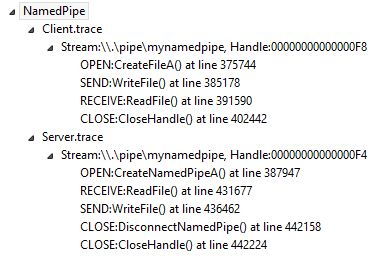
\includegraphics{Figures/result1_streams}}
 \caption{Extracted Streams of $dual\_trace\_1$}
\label{result1_streams}
\end{figure}

The value of the $FileName$ parameter of the $CreateFileA$ function call event in $Client.trace$ is $``.\backslash pipe \backslash mynamepipe"$ as shown in Table \ref{funcclientexp1}. Meanwhile, the value of the $FileName$ parameter of the $CreateNamePipeA$ function call event in $Server.trace$ is also $``.\backslash pipe \backslash mynamepipe"$ as shown in Table \ref{funcserverexp1}. According to the algorithm presented in Section \ref{streammatch}, the file name of a named pipe is treated as the channel identifier which is used to match two streams into a communication. So the stream identified by the handle $0xF8$ in $Client.trace$ is matched to the stream identified by the $0xF4$ in $Server.trace$.

There is only one send event and one receive event in both streams, the data verification of these two matched streams is trivial. Both the concatenation of the sent packet(s) in the stream $0xF8$ of $Client.trace$ and the concatenation of the received packet(s) in the stream $0xF4$ of $Server.trace$ are $``This\; is\; a\; test."$. Both the concatenation of the sent packet(s) in the stream $0xF4$ of $Server.trace$ and the concatenation of the received packet(s) in the stream $0xF8$ of $Client.trace$ are $``This\; is\; the\; answer."$. So these two match streams satisfy the content preservation of the reliable communication. Therefore, they are eventually output as a communication by the ``Communication Identification" operation and listed in the right table of the ``Communication view" in Atlantis as shown in Figure \ref{result1_communications}.


\begin{figure}[H]
\centerline{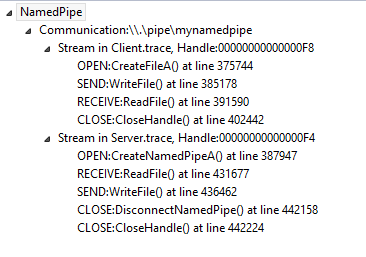
\includegraphics{Figures/result1_communications}}
 \caption{Identified Communication of $dual\_trace\_1$}
\label{result1_communications}
\end{figure}


After seeing the identified communication from $dual\_trace\_1$, I navigated from the send event entries via ``double click" and receive event entries via ``Go To Line of Function End" to the traces. The navigation results are shown in Figures \ref{result1_client_to_server} and \ref{result1_server_to_client}.

\begin{figure}[H]
\begin{subfigure}[H]{0.45\linewidth}
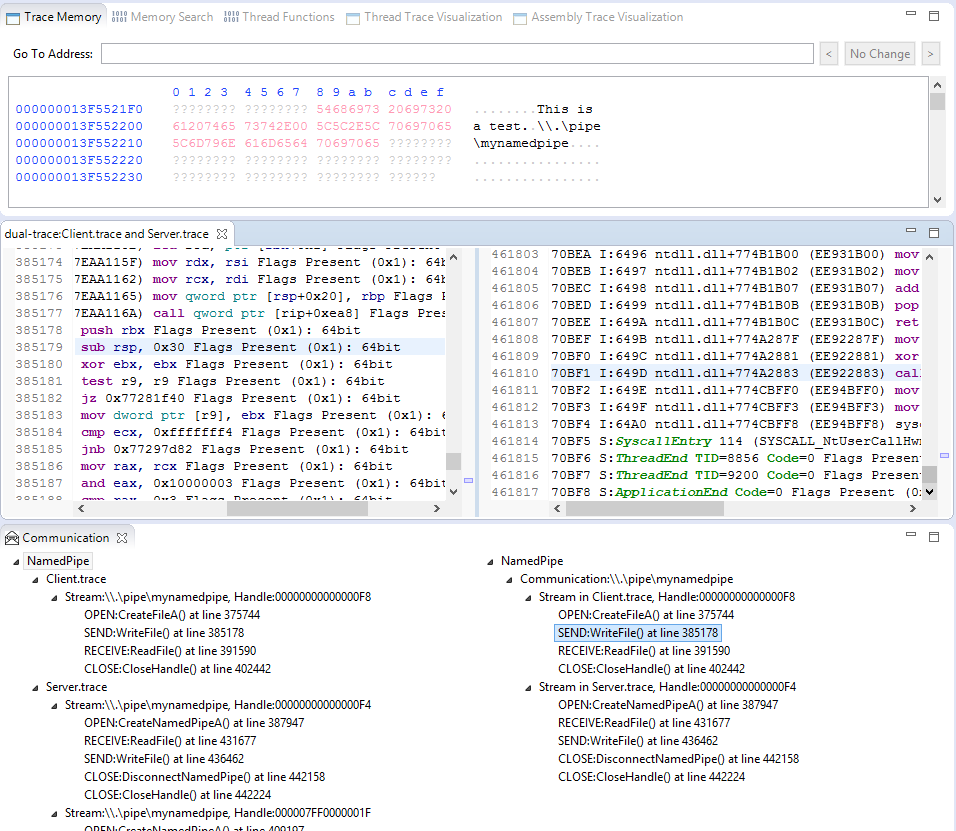
\includegraphics[scale=0.35]{Figures/result1_client_send}
 \caption{Client Send Event Navigation}
\label{result1_client_send}
\end{subfigure}
\hfill
\begin{subfigure}[H]{0.45\linewidth}
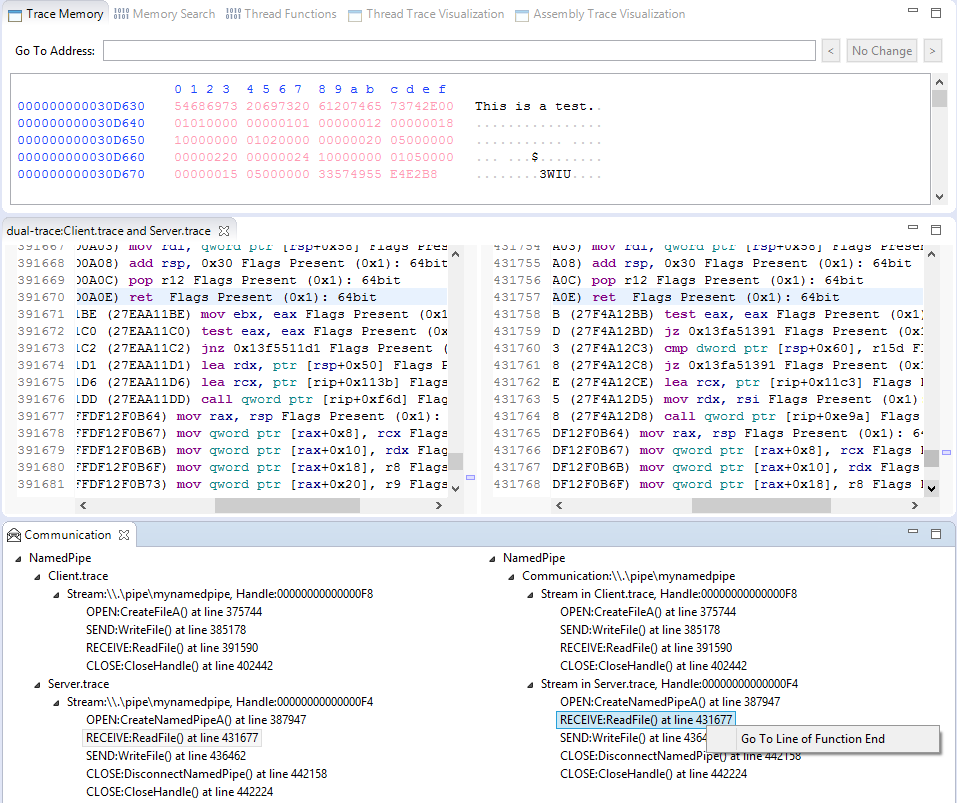
\includegraphics[scale=0.35]{Figures/result1_server_read}
 \caption{Server Receive Event Navigation}
\label{result1_server_read}
\end{subfigure}%
\caption{Navigation Results for the Transmitted Message $``This\; is\; a\; test."$}
\label{result1_client_to_server}
\end{figure}

Figure \ref{result1_client_send} shows when I double clicked on the $WriteFile$ function call event of the $Client.trace$, it brought me to the ``Trace view" of the $Client.trace$ on line 385178 where the function started, and the ``Trace Memory view" jumped to the memory address $0x13F5521F8$, which is the address for the send buffer of the message $``This\; is\; a\; test."$.

Figure \ref{result1_server_read} shows when I selected ``Go To Line of Function End" from the right click menu on the $ReadFile$ function call event of $Server.trace$, that it brought me to the ``Trace view" of $Server.trace$ on line 431757 where the function returned, and the ``Trace Memory view" jumped to the memory address $0x30D630$, which is the address for the receive buffer of the message $``This\; is\; a\; test."$.

These two figures show how the message $``This\; is\; a\; test."$ is transmitted from the client to the server.

\begin{figure}[H]
\begin{subfigure}[H]{0.45\linewidth}
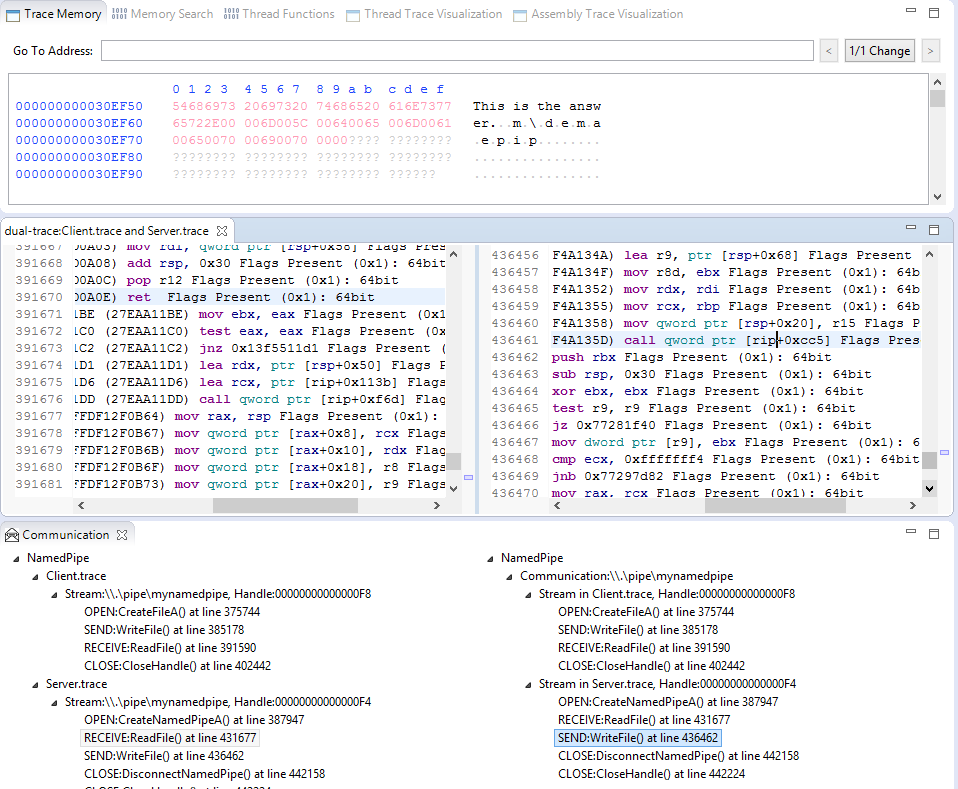
\includegraphics[scale=0.35]{Figures/result1_server_send}
 \caption{Server Send Event Navigation}
\label{result1_server_send}
\end{subfigure}
\hfill
\begin{subfigure}[H]{0.45\linewidth}
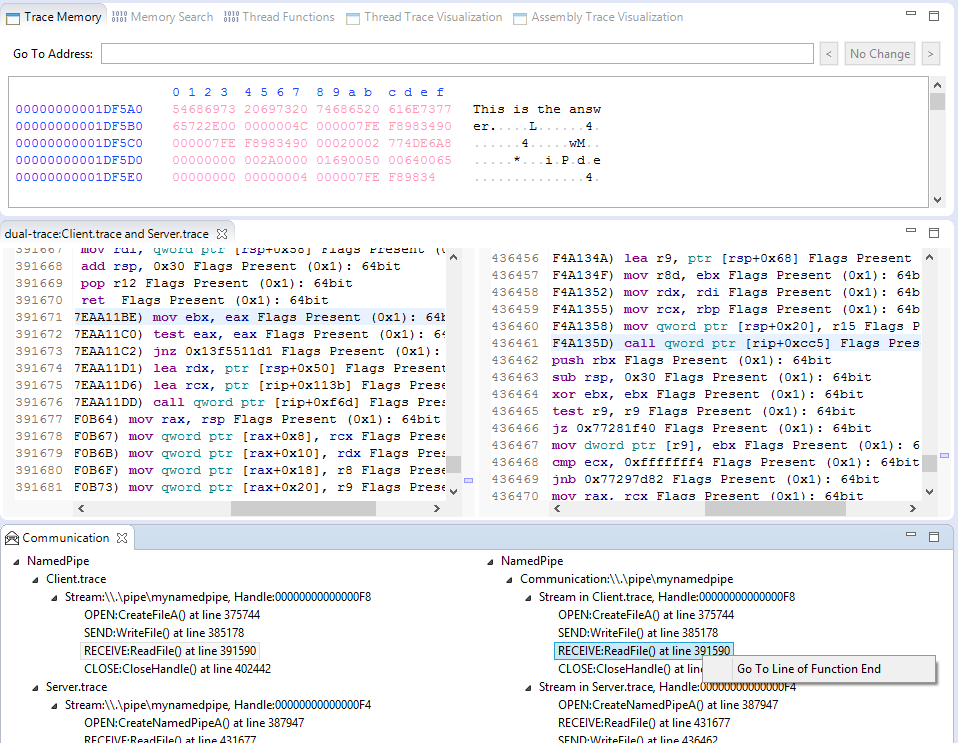
\includegraphics[scale=0.35]{Figures/result1_client_read}
 \caption{Client Receive Event Navigation}
\label{result1_client_read}
\end{subfigure}%
\caption{Navigation Results for the Transmitted Message $``This\; is\; the\; answer."$}
\label{result1_server_to_client}
\end{figure}

Figure \ref{result1_server_send} shows when I double clicked on the $WriteFile$ function call event of $Server.trace$, it brought me to the ``Trace view" of $Server.trace$ on line 436462 where the function started, and the ``Trace Memory view" jumped to the memory address $0x30EF50$, which is the address for the send buffer of the message $``This\; is\; the\; answer."$.

Figure \ref{result1_client_read} shows when I selected ``Go To Line of Function End" in the right click menu on the $ReadFile$ function call event of the $Client.trace$, it brought me to the ``Trace view" of the $Client.trace$ on line 391670 where the function returned, and the ``Trace Memory view" jumped to the memory address $0x1DF5A0$, which is the address for the receive buffer of the message $``This\; is\; the\; answer."$.

These two figures perfectly show how the message $``This\; is\; the\; answer."$ is transmitted from the server to the client.

\section{Experiment 2}
\subsection{Experiment Design}
In the second experiment, one server program and one client program are written in C++. In the server program, four named pipes were created and could be connected by up to four clients at a time. The named pipe client program was run two times in sequence to act as two clients, client1 and client2. Both of these two clients actually connected to the server but sent different messages. Figure \ref{exp2} is the sequence diagram of the interaction among the server and the two clients. This sequence diagram only exemplifies a possible sequence of the events. The actual events sequence can vary depending on the run-time environment. 

Three traces were captured at the time when these three programs were running and interacting with each other. They are $Server.trace$ for the program execution of server , $Client1.trace$ for the program execution of Client 1 and $Client2.trace$ for the program execution of Client 2. These three traces were analyzed as two dual\_traces. The one consisting of $Server.trace$ and $Client1.trace$ is named $dual\_trace\_21$. The other consisting of $Server.trace$ and $Client2.trace$ is named as $dual\_trace\_22$. I performed the ``Stream Extraction" and ``Communication Identification" operations for these two dual\_traces with the function descriptor in Table \ref{fdescexp2}.

\begin{figure}[H]
\centerline{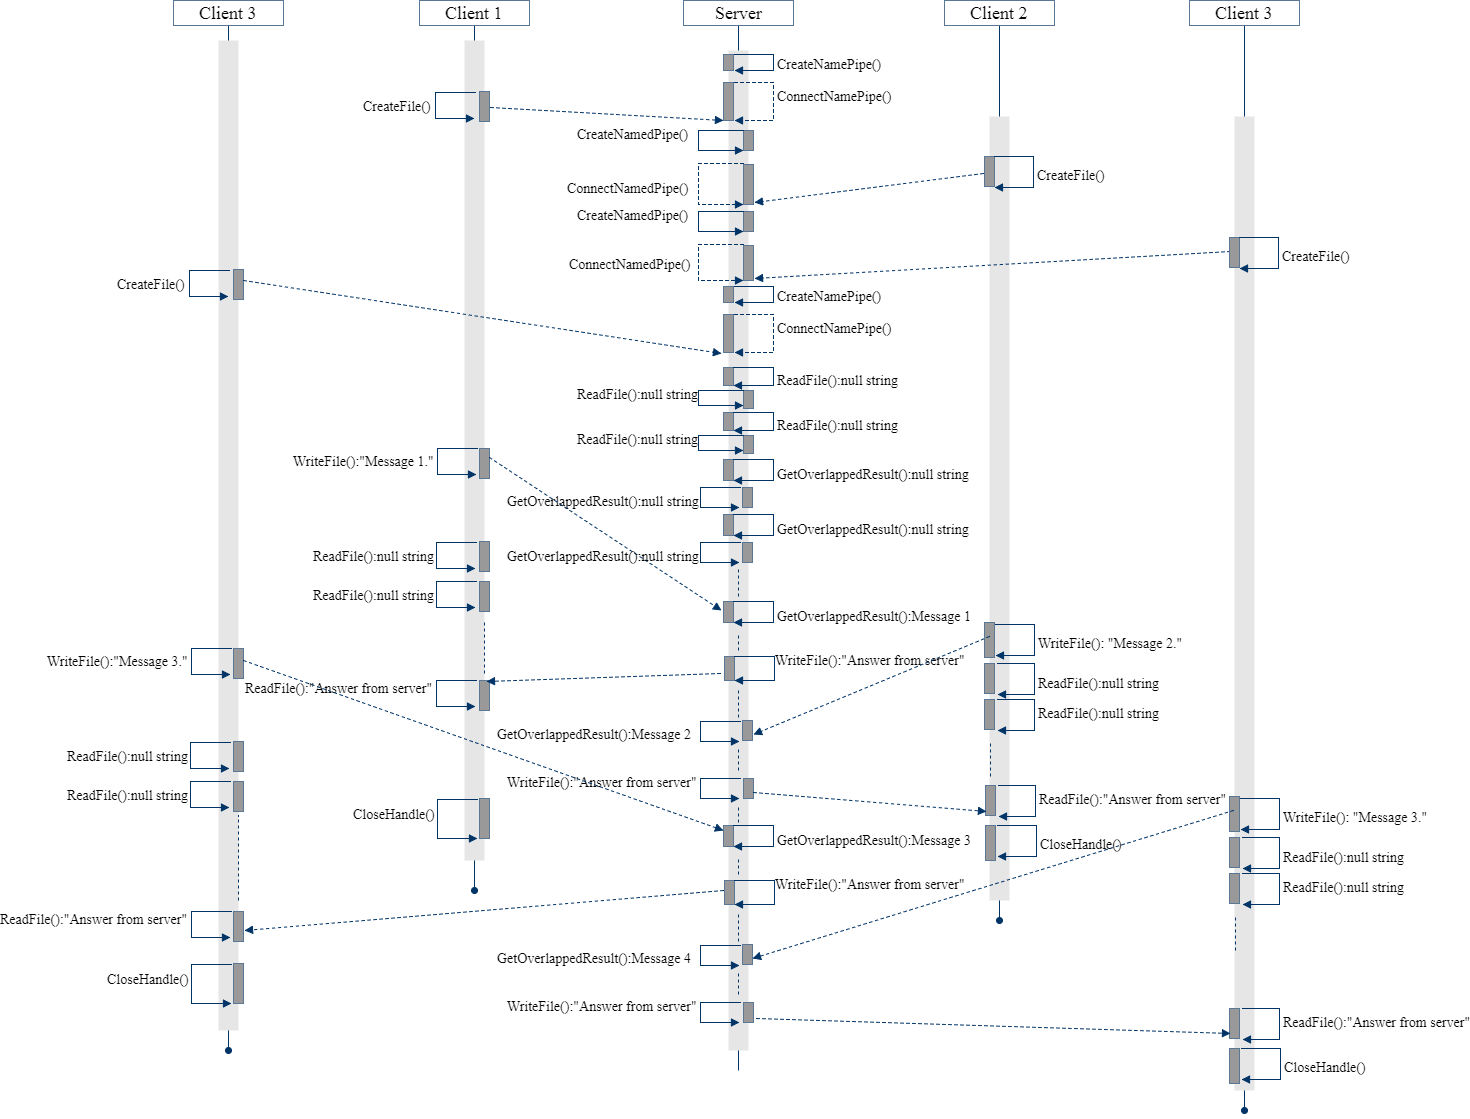
\includegraphics[scale=0.55]{Figures/exp2}}
 \caption{Sequence Diagram of Experiment 2}
\label{exp2}
\end{figure}


\begin{table}[H]
  \centering
  \caption{Function Descriptor of Named Pipe for Experiment 2}
  \label{fdescexp2}
\begin{tabular}{|l|l|l|l|l|l|l|l|}
\hline
             \multirow{2}{*}{{\textbf{Name}}} & \multirow{2}{*}{{\textbf{Type}}} & \multicolumn{3}{c|}{\textbf{Input Parameters Description}} & \multicolumn{3}{c|}{\textbf{Output Parameters Description}} \\
              \cline{3-8} 
             & & \textbf{Name}& \textbf{Register} & \textbf{Addr/Val} & \textbf{Name}& \textbf{Register} &  \textbf{Addr/Val}  \\
             \hline
      CreateNamedPipe
       &open & FileName & RCX  & Addr &  Handle & RAX & Val\\
      \hline         
      CreateFile
       &open & FileName & RCX & Addr&  Handle & RAX & Val\\ 
      \hline              
      \multirow{2}{*}{WriteFile}
       &\multirow{2}{*}{send} &  Handle & RCX & Val & Length & R9 & Val\\
        \cline{3-8} 
       & & SendBuf & RDX & Addr & RetVal& RAX & Val\\
      \hline            
      \multirow{2}{*}{ReadFile}
       &\multirow{2}{*}{receive} &  Handle & RCX & Val& Length & R9 & Val\\
        \cline{3-8} 
       & & RecvBuf & RDX  & Addr & RetVal& RAX & Val\\
      \hline    
           \multirow{2}{*}{GetOverlappedResult} &
       \multirow{2}{*}{receive} &  \multirow{2}{*}{Handle} & \multirow{2}{*}{RCX} & \multirow{2}{*}{Val} &OverlapStruct &RDX & Addr\\
               \cline{6-8} 
       & &  &   &  & RetVal& RAX & Val\\
      \hline     
      CloseHandle &
       close &  Handle & RCX & Val & RetVal& RAX & Val\\
      \hline            
      DisconnectNamedPipe &
      close &  Handle & RCX & Val & RetVal& RAX & Val\\
      \hline               
  \end{tabular}  
\end{table} 

\subsection{Dual\_trace Analysis Result Walk Through}
In this section, I will first walk through the function call event reconstruction and stream extraction results for each traces: $Server.trace$, $Client1.trace$ and $Client2.trace$. Then I will walk through the communication identification results for each dual\_traces: $dual\_trace\_21$ and $dual\_trace\_22$.

\subsubsection{$\boldsymbol{Server.trace:}$}
$Server.trace$ has 1,789,627 instruction lines. Twelve function call events were reconstructed from this trace as listed in Table \ref{funcserverexp1}.

\begin{table}[H]
  \centering
  \tiny
  \caption{The sequence of function call events of $Server.trace$}
  \label{funcserverexp2}
  \begin{tabular}{|l|p{16cm}|}
  \hline
\textbf{Line} & \multicolumn{1}{>{\centering\arraybackslash}m{16cm}|}{\textbf{Event}}\\
  \hline
  1732413 & $funN:CreateNamedPipeA,  type:open, inparams:\lbrace Handle:0x118, FileName:``\dot \backslash pipe \backslash mynamepipe" \rbrace, outparams:\lbrace RetVal:0 \rbrace$\\
 \hline
   1741477 & $funN:CreateNamedPipeA,  type:open, inparams:\lbrace Handle:0x120, FileName:``\dot \backslash pipe \backslash mynamepipe" \rbrace, outparams:\lbrace RetVal:0 \rbrace$\\
 \hline
   1749553 & $funN:CreateNamedPipeA,  type:open, inparams:\lbrace Handle:0x128, FileName:``\dot \backslash pipe \backslash mynamepipe" \rbrace, outparams:\lbrace RetVal:0 \rbrace$\\
 \hline
   1757626 & $funN:CreateNamedPipeA,  type:open, inparams:\lbrace Handle:0x130, FileName:``\dot \backslash pipe \backslash mynamepipe" \rbrace, outparams:\lbrace RetVal:0 \rbrace$\\
 \hline
   1765903 & $funN:GetOverlappedResult, type:receive, inparams:\lbrace Handle:0x118 \rbrace, outparams: \lbrace OverlapStruct:``", RetVal:0\rbrace$\\
\hline
  1765950&$funN:ReadFile, type:receive, inparams: \lbrace Handle:0x118 \rbrace, outparams: \lbrace RecvBuf:``Message\: 2", Length:10, RetVal:0 \rbrace$\\
\hline
  1770738 & $funN:WriteFile, type:send, inparams:\lbrace Handle:0x118, SendBuf:``Default\: answer\: from\: server"\rbrace, outparams: \lbrace Length:20 \rbrace$\\
\hline
   1771629 & $funN:GetOverlappedResult, type:receive, inparams:\lbrace Handle:0x120 \rbrace, outparams: \lbrace OverlapStruct:``", RetVal:0\rbrace$\\
\hline
  1771676&$funN:ReadFile, type:receive, inparams: \lbrace Handle:0x120 \rbrace, outparams: \lbrace RecvBuf:``Message\: 1", Length:10, RetVal:0 \rbrace$\\
\hline
  1775507 & $funN:WriteFile, type:send, inparams:\lbrace Handle:0x120, SendBuf:``Default\: answer\: from\: server"\rbrace, outparams: \lbrace Length:20 \rbrace$\\
\hline
 1777180&$funN:DisconnectNamedPipe, type:close, inparams: \lbrace Handle:0x118 \rbrace, outparams: \lbrace RetVal:0 \rbrace$\\
\hline   
 1778658&$funN:DisconnectNamedPipe, type:close, inparams: \lbrace Handle:0x120 \rbrace, outparams: \lbrace RetVal:0 \rbrace$\\
\hline               
  \end{tabular}
\end{table}

There are four handle values in this event sequence: $0x118$, $0x120$, $0x128$, $0x130$. So four streams are extracted with these four handle identifiers. Both stream $0x118$ and $0x120$ have five events while stream $0x128$ and $0x130$ only have one channel open event. The extracted streams were listed in the left table  of ``Communication view"  as shown in Figure \ref{result21_streams}.

\begin{figure}[H]
\centerline{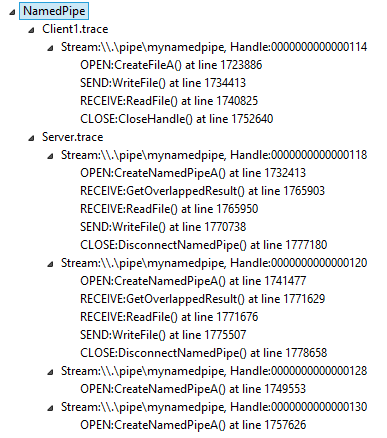
\includegraphics{Figures/result21_streams}}
 \caption{Extracted Streams of $dual\_trace\_21$}
\label{result21_streams}
\end{figure}

\subsubsection{$\boldsymbol{Client1.trace:}$}
$Client1.trace$ has 1,764,281 instruction lines. Four function call events were reconstructed from this trace as listed in Table \ref{funcclient1exp2}.

\begin{table}[H]
  \centering
  \tiny
  \caption{The sequence of function call events of $Client1.trace$}
  \label{funcclient1exp2}
  \begin{tabular}{|l|p{16cm}|}
  \hline
\textbf{Line} & \multicolumn{1}{>{\centering\arraybackslash}m{16cm}|}{\textbf{Event}}\\
  \hline
  1723886 & $funN:CreateFileA,  type:open, inparams:\lbrace Handle:0x114, FileName:``\dot \backslash pipe \backslash mynamepipe" \rbrace, outparams:\lbrace RetVal:0 \rbrace$\\
 \hline
  1734413 & $funN:WriteFile, type:send, inparams:\lbrace Handle:0x114, SendBuf:``Message\:1"\rbrace, outparams: \lbrace Length:15 \rbrace$\\
\hline
 1740825&$funN:ReadFile, type:receive, inparams: \lbrace Handle:0x114 \rbrace, outparams: \lbrace RecvBuf:``Default\; answer\; from \; server", Length:17, RetVal:0 \rbrace$\\
\hline
 1752640&$funN:CloseHandle, type:close, inparams: \lbrace Handle:0x114 \rbrace, outparams: \lbrace RetVal:0 \rbrace$\\
\hline               
  \end{tabular}
\end{table}

All the values of the handle parameter of these four events are $0x114$. So that a stream identified by the handle $0x114$ was extracted, which consists of all these four function call events. The extracted stream was listed in the left table  of ``Communication view"  as shown in Figure \ref{result21_streams}.

\subsubsection{$\boldsymbol{Client2.trace:}$}
$Client2.trace$ has 1764441 instruction lines. Four function call events were reconstructed from this trace as listed in Table \ref{funcclient2exp2}.

\begin{table}[H]
  \centering
  \tiny
  \caption{The sequence of function call events of $Client2.trace$}
  \label{funcclient2exp2}
  \begin{tabular}{|l|p{16cm}|}
  \hline
\textbf{Line} & \multicolumn{1}{>{\centering\arraybackslash}m{16cm}|}{\textbf{Event}}\\
  \hline
  1723886 & $funN:CreateFileA,  type:open, inparams:\lbrace Handle:0x114, FileName:``\dot \backslash pipe \backslash mynamepipe" \rbrace, outparams:\lbrace RetVal:0 \rbrace$\\
 \hline
  1734413 & $funN:WriteFile, type:send, inparams:\lbrace Handle:0x114, SendBuf:``Message\:2"\rbrace, outparams: \lbrace Length:15 \rbrace$\\
\hline
 1740825&$funN:ReadFile, type:receive, inparams: \lbrace Handle:0x114 \rbrace, outparams: \lbrace RecvBuf:``Default\; answer\; from \; server", Length:17, RetVal:0 \rbrace$\\
\hline
 1752800&$funN:CloseHandle, type:close, inparams: \lbrace Handle:0x114 \rbrace, outparams: \lbrace RetVal:0 \rbrace$\\
\hline               
  \end{tabular}
\end{table}

All the values of the handle parameter of these four events are $0x114$. So that a stream identified by the handle $0x114$ was extracted, which consists of all these four function call events. 

\begin{figure}[H]
\centerline{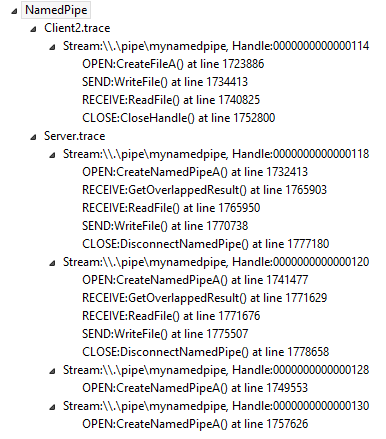
\includegraphics{Figures/result22_streams}}
 \caption{Extracted Streams of $dual\_trace\_22$}
\label{result22_streams}
\end{figure}

\subsubsection{$\boldsymbol{Dual\_trace\_21:}$}
The value of the $FileName$ parameter of the $CreateFileA$ function call event in $Client1.trace$ is $``.\backslash pipe \backslash mynamepipe"$ as shown in Table \ref{funcclient1exp2}. Meanwhile, the values of the $FileName$ parameter of the $CreateNamePipeA$ function call events of all streams in $Server.trace$ are also $``.\backslash pipe \backslash mynamepipe"$ as shown in Table \ref{funcserverexp2}, so that, the stream identified by the handle $0x114$ of $Client.trace$ is matched to all the streams of $Server.trace$.

The send and receive packet contents and the payload concatenation of the streams in the server and client 1 are shown in Table \ref{contentresult21}. Comparing the concatenation of each stream in $Server.trace$, it is obvious that the send payload concatenation of Stream $0x114$ in $Client1.trace$ equals to the receive payload concatenation of Stream $0x120$ in $Server.trace$, while on the other direction, the send payload concatenation of Stream $0x120$ in $Server.trace$ equals to the receive payload concatenation of Stream $0x114$ in $Client1.trace$, so that, only Stream $0x120$ of $Server.trace$ and Stream $0x114$ of $Client1.trace$ satisfy the content preservation of the reliable communication. 

\begin{table}[H]
  \tiny
  \centering
  \caption{Content Summarize of the Extracted Streams}
  \label{contentresult21}
  \begin{tabular}{|l|l|l|l|l|l|}
\hline            
& \multirow{2}{*}{\textbf{Handle}} & \multicolumn{2}{c|}{\textbf{Receive} }&\multicolumn{2}{c|}{\textbf{Send}} \\
\cline{3-6}
& &\multicolumn{1}{c|}{ \textbf{Events} }&\multicolumn{1}{c|}{\textbf{ Concatenation}}&\multicolumn{1}{c|}{ \textbf{Events} }&\multicolumn{1}{c|}{\textbf{ Concatenation}}\\
\hline 
\multirow{6}{*}{$\boldsymbol{Server.trace}$} &\multirow{2}{*}{$0x118$} & $GetOverlappedResult:``"$ & \multirow{2}{*}{$``Message\; 2"$} & $WriteFile:``Default\; "$ &  $``Default\; answer\; "$\\
\cline{3-3}
& &$ReadFile:``Message\; 2"$ &  & $answer\; from\; server"$&$from\; server"$\\
\cline{2-6}    
      &\multirow{2}{*}{$0x120$} & $GetOverlappedResult:``"$ & \multirow{2}{*}{$``Message\; 1"$} & $WriteFile:``Default\; $ &  $``Default\; answer\; "$\\
\cline{3-3}
& &$ReadFile:``Message\; 1"$ & &$answer\; from\; server"$ &$from\; server"$\\  
\cline{2-6}   
& $0x128$&\multicolumn{1}{c|}{- }&\multicolumn{1}{c|}{- } &\multicolumn{1}{c|}{- } &\multicolumn{1}{c|}{- }\\  
\cline{2-6}   
& $0x130$&\multicolumn{1}{c|}{- } &\multicolumn{1}{c|}{- } &\multicolumn{1}{c|}{- } &\multicolumn{1}{c|}{- }\\      
\hline  
\multirow{2}{*}{$\boldsymbol{Client1.trace}$ }&\multirow{2}{*}{$0x114$ }& $ReadFile: ``Default\; $ & $``Default\; answer\; $ & \multirow{2}{*}{$WriteFile:``Message\; 1"$ } &  \multirow{2}{*}{$``Message\; 1"$}\\
& &$answer\; from\; server"$& $ from\; server"$ & &\\
\hline
  \end{tabular}
\end{table}

Therefore, Stream $0x120$ of $Server.trace$ and Stream $0x114$ of $Client1.trace$ are eventually output as a communication by the ``Communication Identification" operation in the right table of ``Communication view" as shown in Figure \ref{result21_communications}. 

\begin{figure}[H]
\centerline{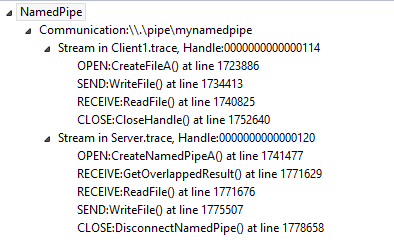
\includegraphics{Figures/result21_communications}}
 \caption{Identified Communication of $dual\_trace\_21$}
\label{result21_communications}
\end{figure}

After I received the identified communication from $dual\_trace\_21$, I navigated from the send and receive events back to the traces. The navigation results are shown in Figure \ref{result21_server_readnull},  Figure \ref{result21_client_to_server} and Figure \ref{result21_server_to_client}.

\begin{figure}[H]
\centerline{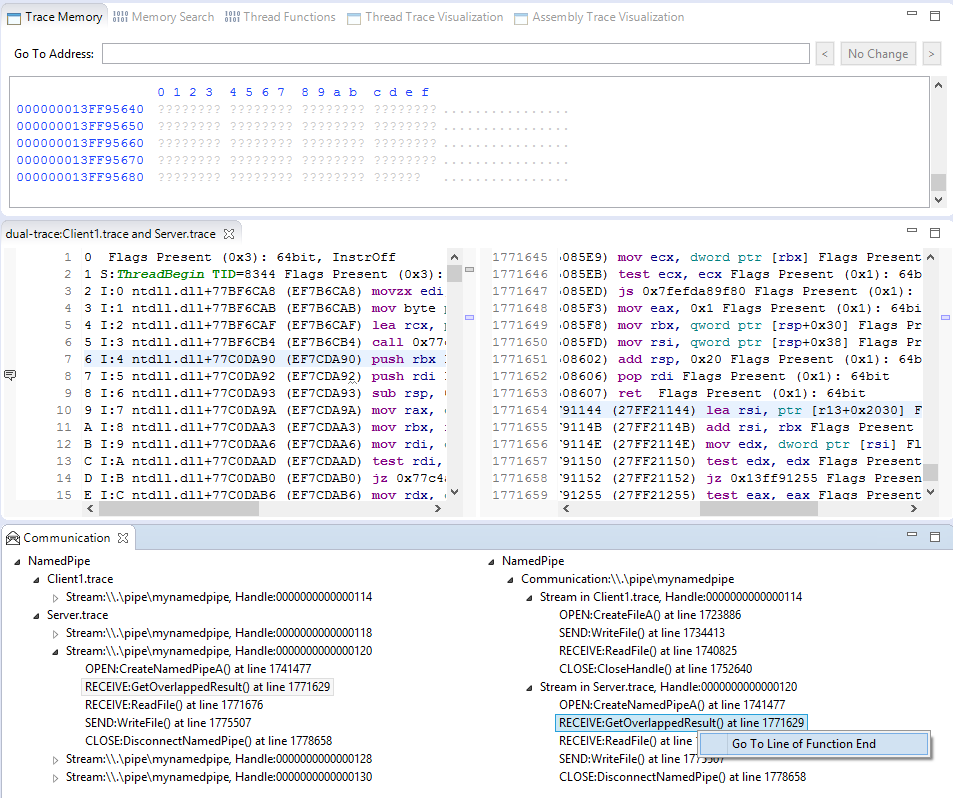
\includegraphics[scale=0.35]{Figures/result21_server_readnull}}
 \caption{Navigation Result for the Function Call Event: $GetOverlappedResult$}
\label{result21_server_readnull}
\end{figure}

Figure \ref{result21_server_readnull} shows when I selected ``Go To Line of Function End" in the right click menu on the $GetOverlappedResult$ function call event of the $Server.trace$, it brought me to the ``Trace view" of the $Server.trace$ on line 1771653 where the function returned. However, since this function call didn't get any message, the ``Trace Memory view" is blank.


\begin{figure}[H]
\begin{subfigure}[H]{0.45\linewidth}
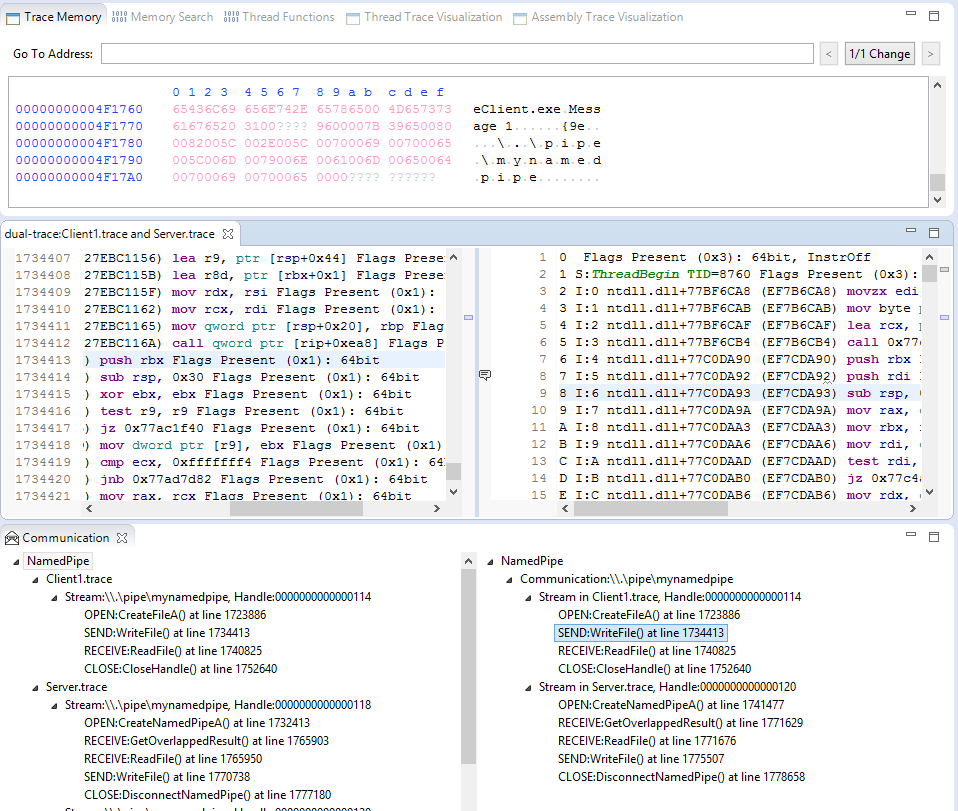
\includegraphics[scale=0.35]{Figures/result21_client_send}
 \caption{Client 1 Send Event Navigation}
\label{result21_client_send}
\end{subfigure}
\hfill
\begin{subfigure}[H]{0.45\linewidth}
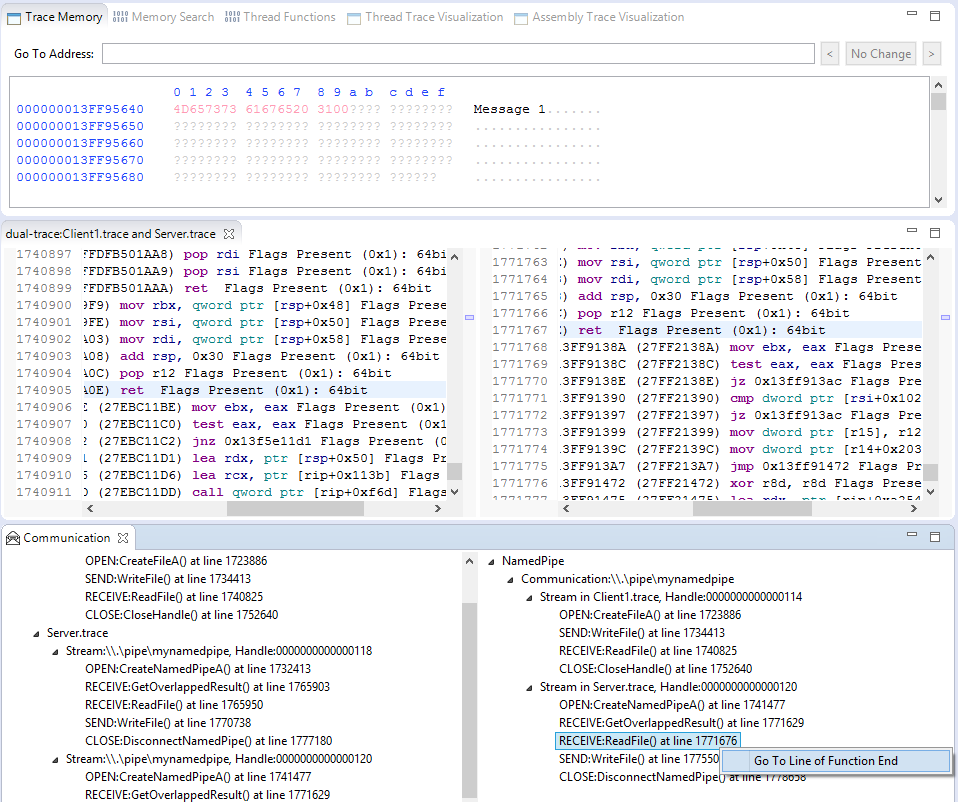
\includegraphics[scale=0.35]{Figures/result21_server_read}
 \caption{Sever Receive Event Navigation}
\label{result21_server_read}
\end{subfigure}%
\caption{Navigation Results for the Transmitted Message $``Message\; 1"$}
\label{result21_client_to_server}
\end{figure}

Figure \ref{result21_client_send} shows when I double clicked on the $WriteFile$ function call event of $Client.trace$, it brought me to the ``Trace view" of $Client.trace$ on line 1734413 where the function started, and the ``Trace Memory view" jumped to the memory address $0x4F176c$, which is the address for the send buffer of the message $``Message\; 1"$.

Figure \ref{result21_server_read} shows when I selected ``Go To Line of Function End" in the right click menu on the $ReadFile$ function call event of the $Server.trace$, it brought me to the ``Trace view" of the $Server.trace$ on line 1771767 where the function returned, and the ``Trace Memory view" jumped to the memory address $0x13FF95640$, which is the address for the receive buffer of the message $``Message\; 1"$.

This two figures perfectly show how the message $``Message\; 1"$ is transmitted from the client 1 to the server.

\begin{figure}[H]
\begin{subfigure}[H]{0.45\linewidth}
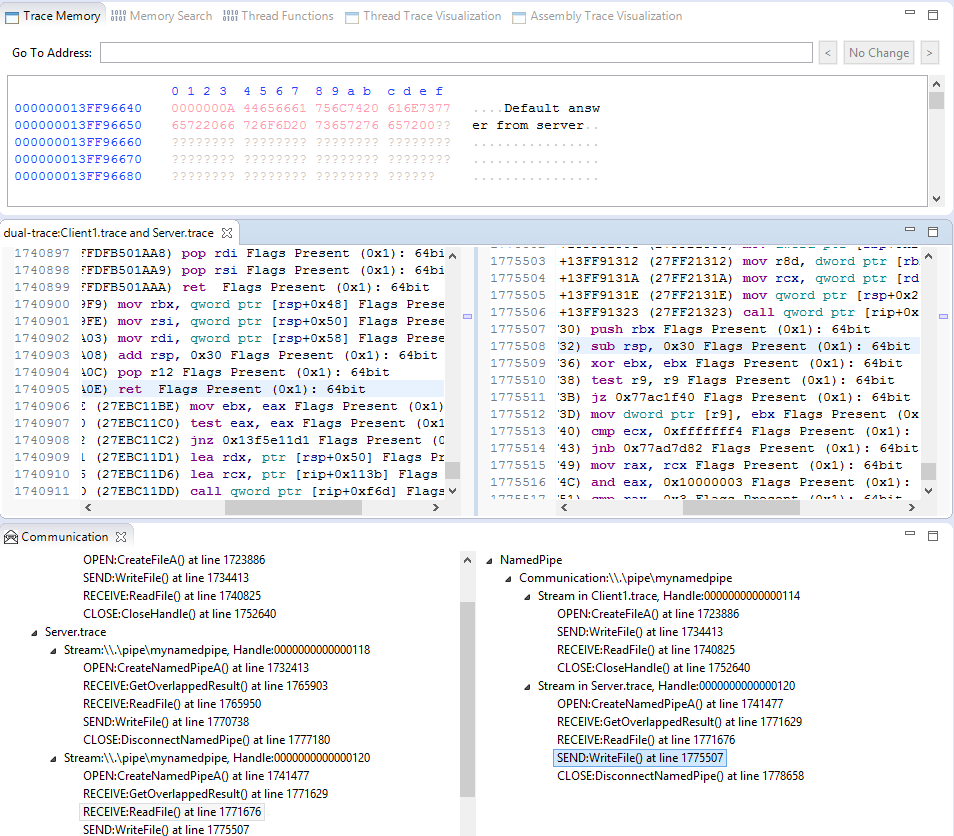
\includegraphics[scale=0.35]{Figures/result21_server_send}
 \caption{Server Send Event Navigation}
\label{result21_server_send}
\end{subfigure}
\hfill
\begin{subfigure}[H]{0.45\linewidth}
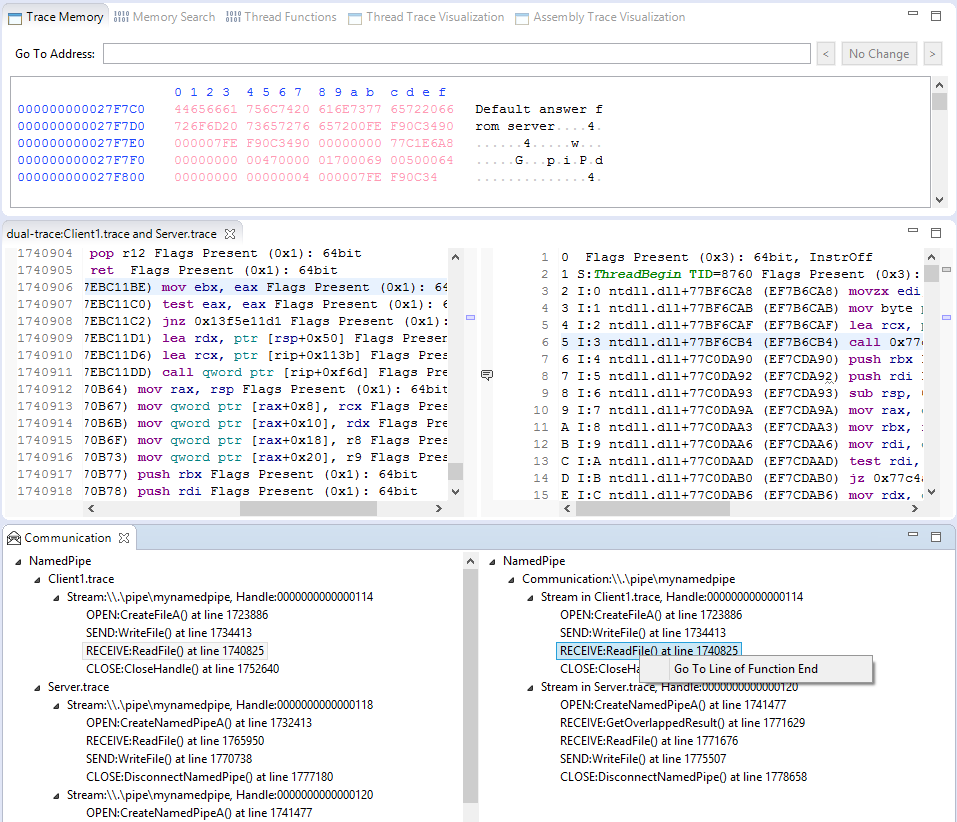
\includegraphics[scale=0.35]{Figures/result21_client_read}
 \caption{Client 1 Receive Event Navigation}
\label{result21_client_read}
\end{subfigure}%
\caption{Navigation Results for the Transmitted Message $``Default\; answer\; from\; server"$}
\label{result21_server_to_client}
\end{figure}

Figure \ref{result21_server_send} shows when I double clicked on the $WriteFile$ function call event of $Server.trace$, it brought me to the ``Trace view" of $Server.trace$ on line 1775507 where the function started, and the ``Trace Memory view" jumped to the memory address $0x30EF50$, which is the address for the send buffer of the message $``Default\; answer\; from\; server"$.

Figure \ref{result21_client_read} shows when I selected ``Go To Line of Function End" in the right click menu on the $ReadFile$ function call event of $Client.trace$, it brought me to the ``Trace view" of $Client.trace$ on line 1740905 where the function returned, and the ``Trace Memory view" jumped to the memory address $0x1DF5A0$ of the receive buffer of the message $``Default\; answer\; from\; server"$.

This two figures perfectly show how the message $``Default\; answer\; from\; server"$ is transmitted from the server to the client 1.

\subsubsection{$\boldsymbol{Dual\_trace\_22:}$}
Similar to $dual\_trace\_22$, all streams of $Server.trace$ will be matched to only one stream of $Client2.trace$ by the stream matching algorithm.

The send and receive packet contents and the payload concatenation of the streams in the server and client 1 are listed in Table \ref{contentresult22}. Comparing the concatenation of each stream in $Server.trace$, it is obvious that the send payload concatenation of Stream $0x114$ in $Client2.trace$ equals the receive payload concatenation of Stream $0x118$ in $Server.trace$, while in the other direction, the send payload concatenation of Stream $0x118$ in $Server.trace$ equals to the receive payload concatenation of Stream $0x114$ in $Client2.trace$, so that, only Stream $0x118$ of $Server.trace$ and Stream $0x114$ of $Client2.trace$ satisfy the content preservation of the reliable communication. 

\begin{table}[H]
  \tiny
  \centering
  \caption{Content Summarize of the Extracted Streams}
  \label{contentresult22}
  \begin{tabular}{|l|l|l|l|l|l|}
\hline            
& \multirow{2}{*}{\textbf{Handle}} & \multicolumn{2}{c|}{\textbf{Receive} }&\multicolumn{2}{c|}{\textbf{Send}} \\
\cline{3-6}
& &\multicolumn{1}{c|}{ \textbf{Events} }&\multicolumn{1}{c|}{\textbf{ Concatenation}}&\multicolumn{1}{c|}{ \textbf{Events} }&\multicolumn{1}{c|}{\textbf{ Concatenation}}\\
\hline 
\multirow{6}{*}{$\boldsymbol{Server.trace}$} &\multirow{2}{*}{$0x118$} & $GetOverlappedResult:``"$ & \multirow{2}{*}{$``Message\; 2"$} & $WriteFile:``Default\; "$ &  $``Default\; answer\; "$\\
\cline{3-3}
& &$ReadFile:``Message\; 2"$ &  & $answer\; from\; server"$&$from\; server"$\\
\cline{2-6}    
      &\multirow{2}{*}{$0x120$} & $GetOverlappedResult:``"$ & \multirow{2}{*}{$``Message\; 1"$} & $WriteFile:``Default\; $ &  $``Default\; answer\; "$\\
\cline{3-3}
& &$ReadFile:``Message\; 1"$ & &$answer\; from\; server"$ &$from\; server"$\\  
\cline{2-6}   
& $0x128$&\multicolumn{1}{c|}{- }&\multicolumn{1}{c|}{- } &\multicolumn{1}{c|}{- } &\multicolumn{1}{c|}{- }\\  
\cline{2-6}   
& $0x130$&\multicolumn{1}{c|}{- } &\multicolumn{1}{c|}{- } &\multicolumn{1}{c|}{- } &\multicolumn{1}{c|}{- }\\      
\hline  
\multirow{2}{*}{$\boldsymbol{Client2.trace}$ }&\multirow{2}{*}{$0x114$ }& $ReadFile: ``Default\; $ & $``Default\; answer\; $ & \multirow{2}{*}{$WriteFile:``Message\; 2"$ } &  \multirow{2}{*}{$``Message\; 2"$}\\
& &$answer\; from\; server"$& $ from\; server"$ & &\\
\hline
  \end{tabular}
\end{table}



Therefore, Stream $0x118$ of $Server.trace$ and Stream $0x114$ of $Client2.trace$ are eventually output as a communication by the ``Communication Identification" operation in the right table of ``Communication view" as shown in Figure \ref{result22_communications}. 

\begin{figure}[H]
\centerline{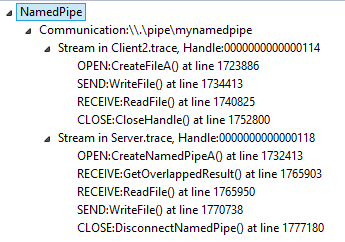
\includegraphics{Figures/result22_communications}}
 \caption{Identified Communication of $dual\_trace\_22$}
\label{result22_communications}
\end{figure}

After I received the identified communication from $dual\_trace\_22$, I navigated from the send and receive events back to the traces. The navigation results are shown in Figure \ref{result22_server_readnull}, Figure \ref{result22_client_to_server} and Figure \ref{result22_server_to_client}.

\begin{figure}[H]
\centerline{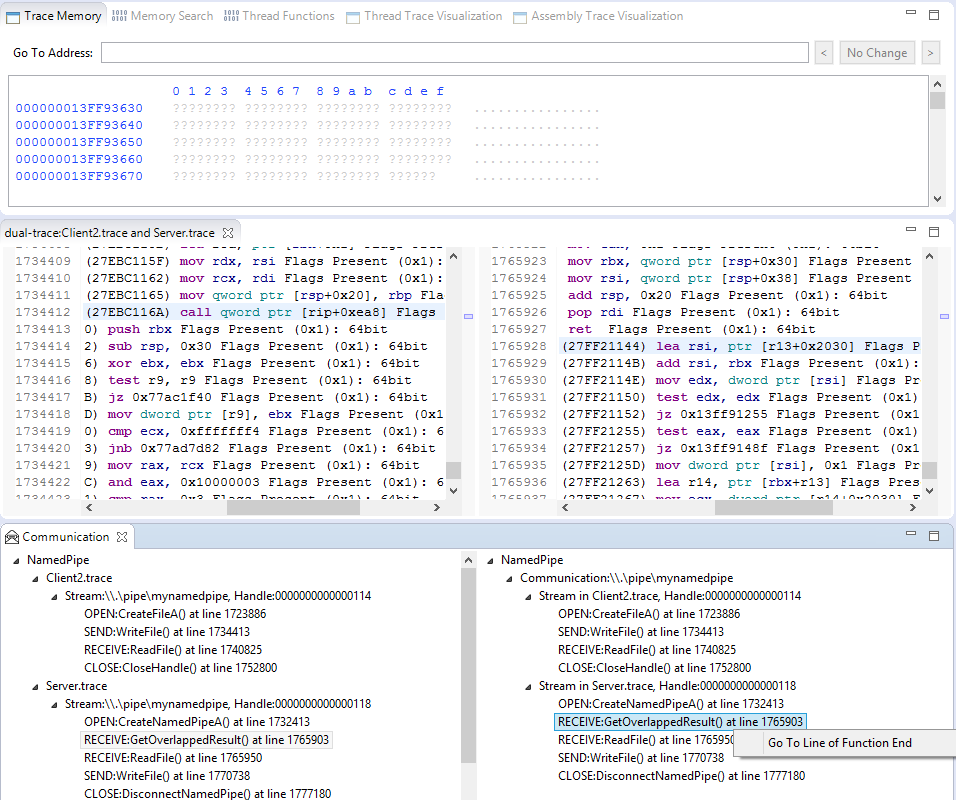
\includegraphics[scale=0.35]{Figures/result22_server_readnull}}
 \caption{Navigation Result for the Function Call Event: $GetOverlappedResult$}
\label{result22_server_readnull}
\end{figure}

Figure \ref{result22_server_readnull} shows when I selected ``Go To Line of Function End" in the right click menu on the $GetOverlappedResult$ function call event of the $Server.trace$, it brought me to the ``Trace view" of the $Server.trace$ on line 1765927 where the function returned. However, since this function call didn't get any message, the ``Trace Memory view" is blank.

\begin{figure}[H]
\begin{subfigure}[H]{0.45\linewidth}
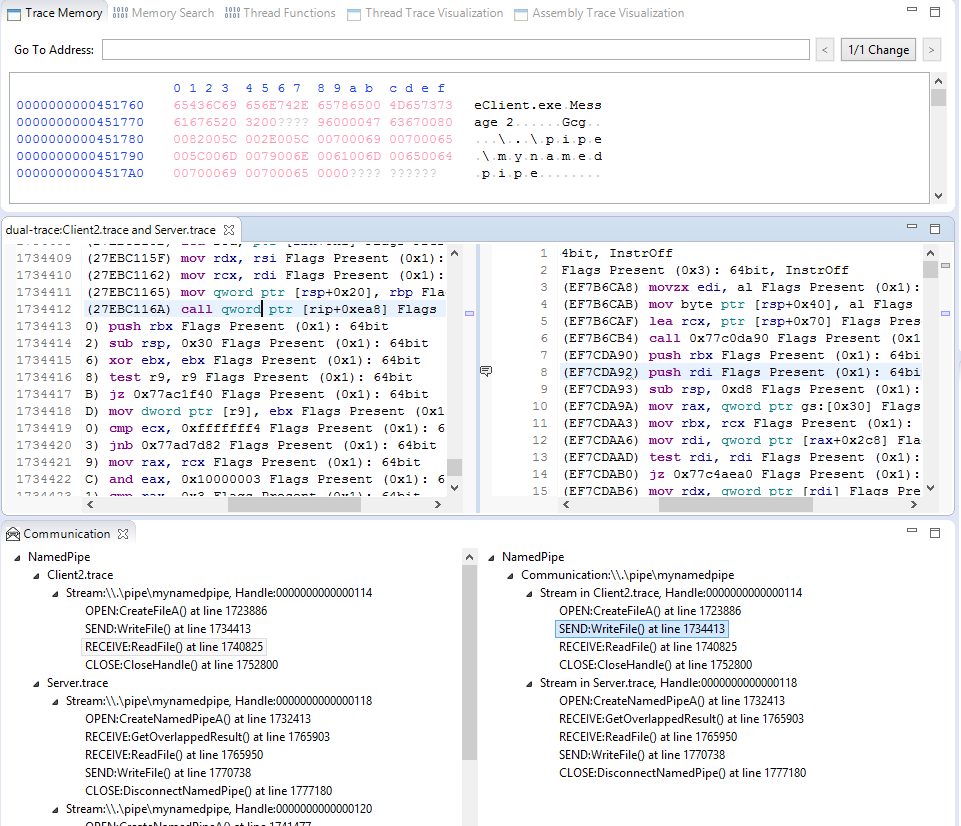
\includegraphics[scale=0.35]{Figures/result22_client_send}
 \caption{Client 2 Send Event Navigation}
\label{result22_client_send}
\end{subfigure}
\hfill
\begin{subfigure}[H]{0.45\linewidth}
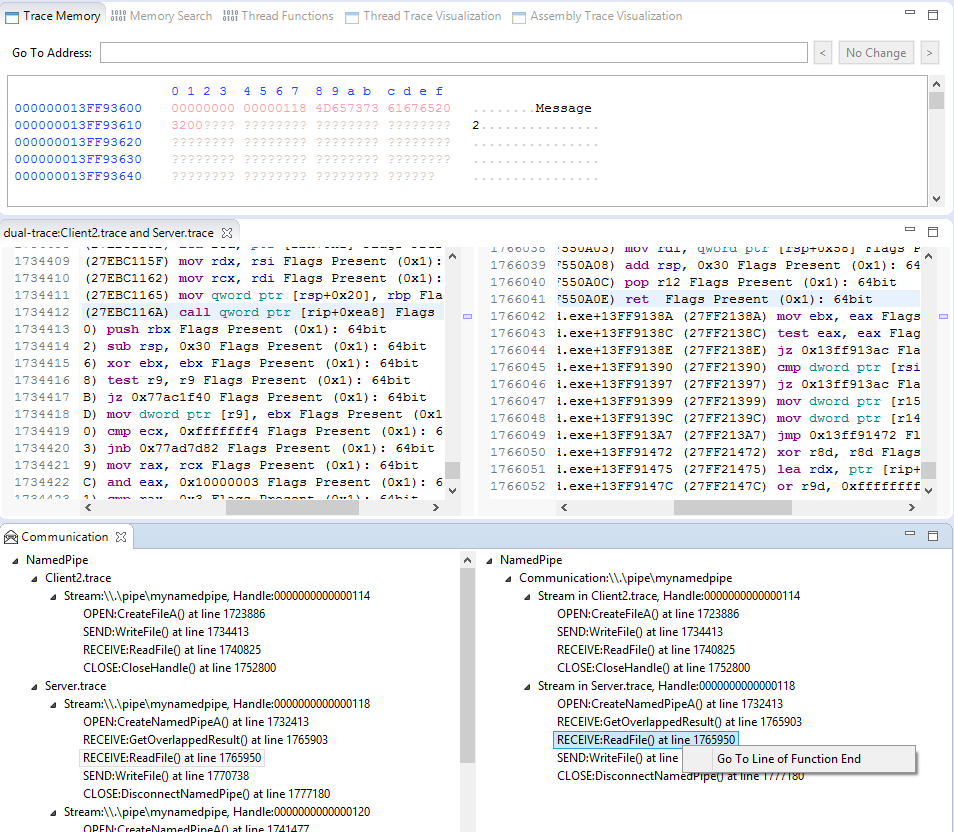
\includegraphics[scale=0.35]{Figures/result22_server_read}
 \caption{Sever Receive Event Navigation}
\label{result22_server_read}
\end{subfigure}%
\caption{Navigation Results for the Transmitted Message $``Message\; 2"$}
\label{result22_client_to_server}
\end{figure}

Figure \ref{result22_client_send} shows when I double clicked on the $WriteFile$ function call event of $Client.trace$, it brought me to the ``Trace view" of $Client.trace$ on line 1734413 where the function started, and the ``Trace Memory view" jumped to the memory address $0x45176c$, which is the address for the send buffer of the message $``Message\; 2"$.

Figure \ref{result22_server_read} shows when I selected ``Go To Line of Function End" in the right click menu on the $ReadFile$ function call event of the $Server.trace$, it brought me to the ``Trace view" of the $Server.trace$ on line 1766041 where the function returned, and the ``Trace Memory view" jumped to the memory address $0x13FF93608$, which is the address for the receive buffer of the message $``Message\; 2"$.

These two figures show how the message $``Message\; 2"$ is transmitted from the client 2 to the server.


\begin{figure}[H]
\begin{subfigure}[H]{0.45\linewidth}
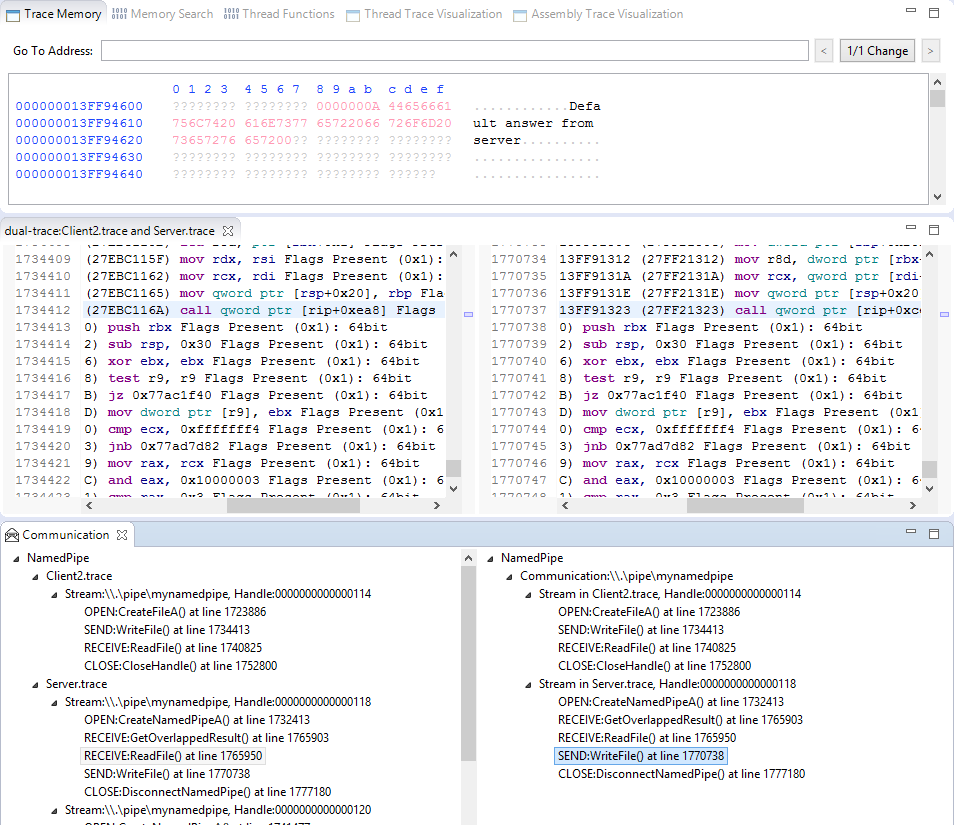
\includegraphics[scale=0.35]{Figures/result22_server_send}
 \caption{Server Send Event Navigation}
\label{result22_server_send}
\end{subfigure}
\hfill
\begin{subfigure}[H]{0.45\linewidth}
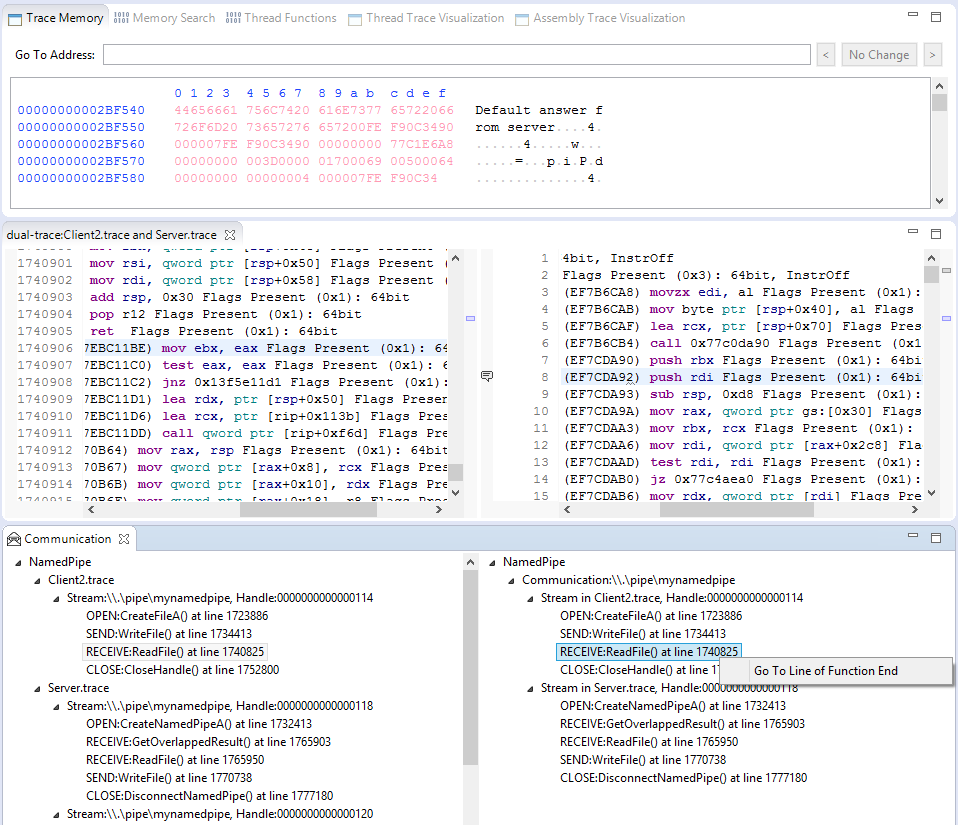
\includegraphics[scale=0.35]{Figures/result22_client_read}
 \caption{Client 2 Receive Event Navigation}
\label{result22_client_read}
\end{subfigure}%
\caption{Navigation Results for the Transmitted Message $``Default\; answer\; from\; server"$}
\label{result22_server_to_client}
\end{figure}

Figure \ref{result22_server_send} shows when I double clicked on the $WriteFile$ function call event of the $Server.trace$, it brought me to the ``Trace view" of the $Server.trace$ on line 1770738 where the function started, and the ``Trace Memory view" jumped to the memory address $0x13FF94608$, which is the address for the send buffer of the message $``Default\; answer\; from\; server"$.

Figure \ref{result22_client_read} shows when I selected ``Go To Line of Function End" in the right click menu on the $ReadFile$ function call event of $Client.trace$, it brought me to the ``Trace view" of $Client.trace$ on line 1740906 where the function returned, and the ``Trace Memory view" jumped to the memory address $0x2BF540$ of the receive buffer of the message $``Default\; answer\; from\; server"$.

These two figures perfectly show how the message $``Default\; answer\; from\; server"$ is transmitted from the server to the client 2.

\section{Conclusion}
By walking through the analysis results of the ``Stream Extraction" and ``Communication Identification" operations in these two experiments, I can conclude that ``Stream Extraction" operation is capable of properly extracting the streams from both traces in a dual\_trace, while ``Communication Identification" operation is capable of identifying the communication between the two traces of a dual\_trace. 

Moreover, from the ``Communication view", the user can easily navigate back to the exact instruction line where the function start or end. The messages transmitted can be shown in the ``Trace Memory view" accurately.

These two experiments are not provided as an empirical evaluation but it shows the usefulness of the algorithms and the prototype implementation.







   




